% vim: set tw=78 sts=2 sw=2 ts=8 aw et ai:

\texttt{BSD} stands for "Berkeley Software Distribution". It is derived from AT\&T's Research UNIX operating system. In 1990, the BSD code was released without the proprietary AT\&T code.
Since the proprietary code contained a good portion of the kernel, it was not until 1992 that a complete operating system based on the BSD code was released - 386BSD. In 1993, the FreeBSD operating system split from the 386BSD project\cite{bsd}. 

\subsection{FreeBSD vs Linux}
\label{subsec:bsdlinux}

While FreeBSD originated from the UNIX systems, Linux was built to be a similar alternative for these. Therefore, they share many mechanisms, tools and applications.

The most significat difference between the two consists in the licensing. Linux is licensed under GNU General Public License(GPL)\cite{gnu}. This allows freedom to modify and redistribute the source code as long as it is also licensed under the GPL. FreeBSD is licensed under the BSD license, which is more permissive. It does not require derived work to maintain the license, but only to include a copy of the BSD license and original copyright\cite{bsd-license}.

Another difference consists of the available software. While most Linux distributions have little to no support for building software from source, FreeBSD provides an extensive collection of software source code which the user can customize and build. Conversely, while BSD maintainers are more conservative when modifying software packages, Linux distribution maintainers make modifications in order to improve component interconnection and management\cite{comp-bsd-linux}.

\subsection{bhyve}
\label{subsec:bhyve}

\texttt{bhyve} is an abbreviation for BSD hypervisor. It is a type-2 hypervisor, similar to Linux KVM. As of FreeBSD 10.0, it is part of the base system. It support various guest systems, ranging from other BSD systems to Linux distributions\cite{intr-bhyve}.

Being a legacy-free hypervisor, it is reliant on the virtualization features of CPUs. It requires both CPU and memory virtualization technologies.

bhyve has several components\cite{intr-bhyve}\cite{extending-bhyve}:
\begin{itemize}
\item
\textbf{vmm.ko} - kernel module, manages VT-x state, context switching, guest physical memory and other aspects
\item
\textbf{libvmmapi} - userland API
\item
\textbf{bhyveload} - userspace bootloader, creates vm and does initial setup, loads guest operating system
\item
\textbf{bhyve} - userspace run loop, emulates stdin/stdout, tap devices, block devices
\item
\textbf{bhyvectl} - utility that can modify virtual machine state; can also delete VMs
\end{itemize}

\begin{figure}[ht]
\centering
  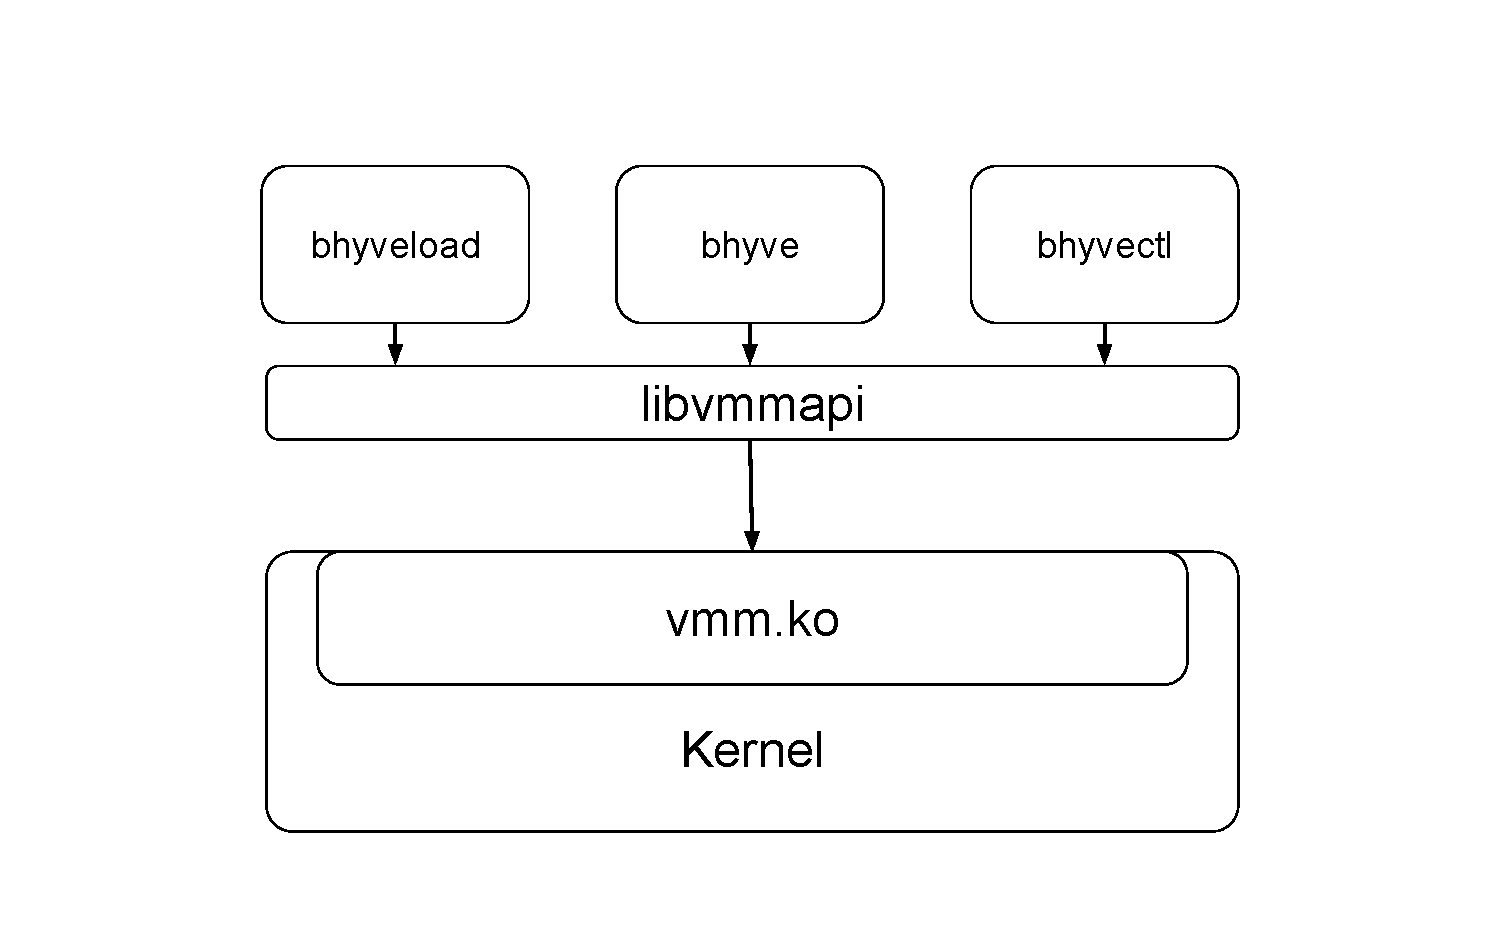
\includegraphics[width=.75\linewidth]{img/bhyve.pdf}
  \caption{bhyve overview}
\end{figure}
